\documentclass[../DC2017114Bouma.tex]{subfiles}
\begin{document}
\graphicspath{{02_Material/img/}}
%% New chapter
\renewcommand{\chaptermark}[1]{\markboth{\thechapter.\ #1}{}}
\renewcommand{\sectionmark}[1]{\markright{#1}{}}
\pagestyle{fancyreport}
\cleartooddpage
\pagestyle{fancyreport}
\chapter{Mechanical Systems with Unilateral Constraints and Spatial Friction}\label{ch:model}
\nomenclature[RD]{$\Db$}{Delassus matrix}%
\nomenclature[Rf]{$\fb$}{A nonlinear continuous function}%
\nomenclature[Rg]{$\gb$}{A jump map}%
\nomenclature[G03]{$\gamma$}{A flow guard function}%
\nomenclature[G03]{$\Gamma$}{An impulsive guard function}%
\nomenclature[G01]{$\alphab$}{The nominal reference trajectory}%
\nomenclature[G12]{$\mub$}{The nominal reference input}%
\nomenclature[S00]{$\dot{(\cdot)}$}{First time derivative}%
\nomenclature[S01]{$\ddot{(\cdot)}$}{Second time derivative}%
\nomenclature[S02]{$(\cdot)^-$}{The left limit}%
\nomenclature[S03]{$(\cdot)^+$}{The right limit}%
\nomenclature[S00]{$(\cdot)_0$}{Initial condition}%
\nomenclature[S04]{$(\cdot)_{\alphab}$}{Related to reference trajectory $\alphab$}%
\nomenclature[S09]{$(\cdot)_{\iota}$}{Related to reference trajectory $\iota$}%
\nomenclature[Sj]{$(\cdot)_{j}$}{Related to event or segment $j$}%
\nomenclature[Si]{$(\cdot)_{i}$}{Related to macro-event or segment $i$}%
\nomenclature[Sk]{$(\cdot)_{k}$}{Related to micro-event or segment $k$}%
\nomenclature[Sx]{$(\cdot)_{\xb}$}{Related to reference trajectory $\xb$}%
\nomenclature[Sn]{$(\cdot)_{n}$}{Scalar or vector in normal direction}%
\nomenclature[St]{$(\cdot)_{t}$}{Scalar or vector in tangential direction}%
In this chapter, several modeling approaches for mechanical systems with unilateral constraints and spatial friction are presented. We start by presenting a general representation of mechanical systems. Then, several formulations of contact and friction laws are introduced in the form of complementarity conditions. The complementarity problem formulation is a complete and often used formulation for mechanical systems with unilateral constraints. This complementarity formulation is then transformed into a hybrid system formulation, that will be used in this work to analyze the tracking of trajectories of mechanical systems with unilateral constraints and spatial friction. While the hybrid system formulation is restrictive in modeling, it is a powerful tool for the control of systems with a special class of trajectories. Since the analysis that will be presented in this work is done with controller design in mind, the analysis will be presented in the hybrid system framework.

\section{General system definition}
When a unilateral constraint is activated, the differential equation that describes the dynamics of the system can change. The state even goes through a reinitialization when the constraint is activated with non-zero velocity. Two bodies already in contact can also experience changes in their dynamics, as a result from the friction between these bodies. This behavior can be described by dynamics consisting of a continuous part and a discrete part; the continuous part describes the flow of the state, and the discrete part describes the reinitialization of the state. The occurrence of a change in differential equation and a possible state reinitialization are referred to as \textit{events}. To be able to detect when the system goes through a such an event, contact points are defined on the bodies. These contact points can activate and deactivate unilateral constraints, which corresponds with opening and closing contact with another body. A contact point that has activated a unilateral constraint can transition between stick and slip. A contact point in stick has a tangential relative velocity of zero, whereas a contact point in stick has a nonzero tangential relative velocity. The \textit{mode} of the contact point is defined. The mode determines if a contact point is in contact or not, and if it is in stick or slip when the contact point is in contact. Using these contact points, a method is presented to model mechanical systems with unilateral constraints and spatial friction. 

Let us now consider a mechanical system whose current configuration is described by the generalized coordinates $\qb\in\mathbb{R}^n$ and whose generalized velocity is denoted $\nub\in\mathbb{R}^n$ with $\nub=\dot{\qb}$ almost everywhere. The configuration space of the system is restricted using $c$ unilateral constraints for modeling contact, using the set of contact points $\mathcal{I}=\{\iota_1,\iota_2,\dots,\iota_c\}$. The set $\Ic_{\text{cl}}$ is defined as the set of $c_{\text{cl}}$ closed contact points, i.e., for a contact $\iota\in\Ic_{\text{cl}}$ the corresponding unilateral constraint is active. The set of potential contact points for which this geometric constraint is inactive, or open contact points, we define as $\Ic_{\text{op}} := \{\iota\ |\ \iota\notin\Ic_{\text{cl}}\}$. Note that in a physics-based engine the set $\Ic_{\text{op}}$ is often undefined, because not all contact points are tracked. Only the contact points generating reaction forces are tracked. The set $\Ic_{\text{op}}$ is only defined for convenience when the mode of the system is discussed. When a unilateral constraint is activated at a nonzero relative velocity, impact happens. For the unilateral constraint not to be violated, a jump in the velocity has to occur. These impact-times are denoted $\tau_j$, where $j\in \{1,2,\dots,N\}$ is a counter for unilateral constraint activations, with $N$ the number of jumps in a trajectory.

Consider Figure~\ref{fig:contactplanes} showing two bodies. A contact point $\iota$ is defined on one of the bodies, at which a plane tangent to the surface of the body is spanned. In the direction normal to this plane, the contact distance $\hrm_{n,\iota}(\qb)$ is defined. The contact distance is the minimal distance between the contact point and the surface that it can make contact with. For the relative normal velocity $\mathrm{v}_{n,\iota}\in\Rbb$ of contact point $\iota$ follows that
\begin{align}
\vrm_{n,\iota} = \frac{\partial \hrm_{n,\iota}}{\partial\qb}\frac{\text{d}\qb}{\text{d} t} = \wb_{n,\iota}^T\dot{\qb},
\end{align}
\nomenclature[G09]{$\iota$}{The contact point counter}%
\nomenclature[Rj]{$j$}{Event counter and hybrid time}%
\nomenclature[Rc]{$c$}{The number of contact points}%
\nomenclature[RN]{$N$}{The number of events}%
\nomenclature[Rw]{$\wb^T_{n,\iota}$}{The normal Jacobian of contact point $\iota$}%
\nomenclature[RW]{$\Wb^T_{t,\iota}$}{The tangential Jacobian of contact point $\iota$}%
\nomenclature[Scl]{$(\cdot)_{\text{cl}}$}{The closed-contact mode sub/superscript}%
\nomenclature[Sop]{$(\cdot)_{\text{op}}$}{The open-contact mode sub/superscript}%
\nomenclature[Ssl]{$(\cdot)_{\text{sl}}$}{The slip-contact mode sub/superscript}%
\nomenclature[Sst]{$(\cdot)_{\text{st}}$}{The stick-contact mode sub/superscript}%
\nomenclature[RI]{$\Ic$}{A set of contact points}%
\nomenclature[Rq]{$\qb$}{The generalized coordinates}%
\nomenclature[Rx]{$\xb$}{The state coordinates}%
\nomenclature[Ru]{$\ub$}{The input}%
\nomenclature[G19]{$\tau$}{The nominal event time}%
\nomenclature[Rt]{$t$}{Regular time}%
\nomenclature[G13]{$\nub$}{The generalized coordinates defined on the continuous segments of a trajectory}%
\nomenclature[Rh]{$\hrm_{n,\iota}$}{Normal contact distance of contact point $\iota$}%
\nomenclature[Rh]{$\hbf_{t,\iota}$}{Tangential contact distance of contact point $\iota$}%
\nomenclature[Rv1]{$\vrm_{n,\iota}$}{Normal velocity of contact point $\iota$}%
\nomenclature[Rv2]{$\vbf_{t,\iota}$}{Tangential velocity of contact point $\iota$}%
with $\wb^T_{n,\iota}\in\Rbb^n$ representing the Jacobian of the normal velocity $\vrm_{n,\iota}$. The relative tangential velocity $\vbf_{t,\iota}\in\Rbb^2$ is defined in the tangent plane of contact point $\iota$. Similar to the normal direction, $\hbf_{t,\iota} = \begin{bmatrix} \hbf_{t_1,\iota} & \hbf_{t_2,\iota} \end{bmatrix}^T$, where $\hbf_{t_1,\iota}$ and $\hbf_{t_2,\iota}$ are the contact distances in $t_1$ direction and $t_2$ direction, respectively. It then follows that the relative tangential velocity is given by
\begin{align}
\vbf_{t,\iota} = \frac{\partial \hbf^T_{t,\iota}}{\partial\qb}\frac{\text{d}\qb}{\text{d} t} = \Wb_{t,\iota}^T\dot{\qb},
\end{align}
with $\Wb^T_{t,\iota}\in\Rbb^{n\times 2}$ representing the Jacobian of the tangential relative velocity $\vbf_{t,\iota}$.
\begin{figure}[bt!]
\centering
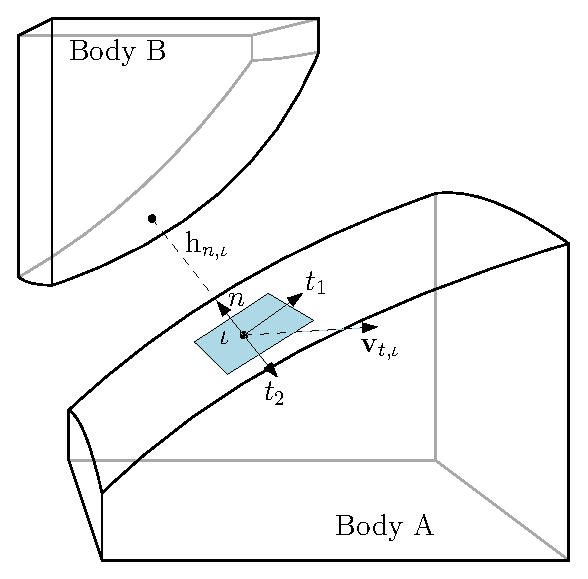
\includegraphics[width=.5\textwidth]{contactplanes2.eps}\caption{An illustration of two bodies about to make contact. The contact distance $\hrm_{n,\iota}$ and the relative tangential velocity $\vbf_{t,\iota}$ for contact point $\iota$ are illustrated, which are defined on the surface of Body A.} \label{fig:contactplanes}
\end{figure}

Then, the continuous dynamics of a mechanical system with unilateral constraints and spatial friction are of the form
\begin{align}
&\Mb(\qb)\dot{\nub} + \Cb(\qb,\nub) = \Sb(\qb)\ub + \sum_{\iota\in\Ic_{\text{cl}}}\wb_{n,\iota}(\qb)\lambda_{n,\iota} + \Wb_{t,\iota}(\qb)\lambdab_{t,\iota}, \label{eq:appcont1}\\
&\text{(Contact Law)},\nonumber\\
&\text{(Friction Law)},\nonumber
\end{align}
\nomenclature[G11]{$\lambda_{n,\iota}$}{The normal reaction force of contact point $\iota$}%
\nomenclature[G11]{$\lambdab_{t,\iota}$}{The tangential reaction force of contact point $\iota$}%
\nomenclature[G11]{$\Lambda_{n,\iota}$}{The normal impulsive reaction force of contact point $\iota$}%
\nomenclature[G11]{$\Lambdab_{t,\iota}$}{The tangential impulsive reaction force of contact point $\iota$}%
\nomenclature[RM]{$\Mb$}{The mass matrix}%
\nomenclature[RC]{$\Cb$}{The column containing centripedal, Coriolis and gravitational effects}%
\nomenclature[RS]{$\Sb$}{The matrix containing generalized directions of the actuator forces}%
with $\qb,\nub\in\Rbb^{n}$ and $\ub\in\Rbb^m$. In \eqref{eq:appcont1}, $\Mb(\qb)\in\Rbb^{n\times n}$ is the mass matrix of the system, $\Cb(\qb,\nub)\in\Rbb^{n}$ contains the centripetal, Coriolis, stiffness and damping related forces, and gravitational forces in the system and $\Sb(\qb)\in\Rbb^{n\times m}$ represents the generalized directions of the input forces $\ub$. $\lambda_{n,\iota}\in\Rbb$ and $\lambdab_{t,\iota}\in\Rbb^{2}$ are the normal and tangential reaction forces, respectively, of contact point $\iota$ with $\wb_{n,\iota}\in\Rbb^{n}$ and $\Wb_{t,\iota}\in\Rbb^{n\times 2}$ the transposed corresponding Jacobians. To make the system description in \eqref{eq:appcont1} complete, a contact law and friction law is required. These laws will be discussed in Section~\ref{sec:comp}.

As mentioned above, when a unilateral constraint is activated, impulsive dynamics can cause a jump in the generalized velocity of the system. The impulsive dynamics, derived in \cite[Section 5.4]{Leine2008}, are of the form

\begin{align}
&\Mb(\qb)(\nub^+ - \nub^-) = \sum_{\iota\in\Ic_{\text{cl}}} \wb_{n,\iota}(\qb)\Lambda_{n,\iota} + \Wb_{t,\iota}(\qb)\Lambdab_{t,\iota}, \label{eq:appimp1}\\
&\text{(Impulsive Contact Law)},\nonumber\\
&\text{(Impulsive Friction Law)},\nonumber
\end{align}
with $\Lambda_{n,\iota}$ and $\Lambdab_{t,\iota}$ the normal and tangential impulsive reaction forces, respectively, of contact point $\iota$. These dynamics are impulsive, and happen at one instance in time. In \eqref{eq:appimp1}, $\nub^-$ and $\nub^+$ denote the left, respectively the right limit of the generalized velocity $\nub$ at the time of impact $\tau_j$. The expression moreover states that, similarly to the continuous dynamics \eqref{eq:appcont1}, constitutive laws for contact and friction are required. These will be discussed in the following. First a complementarity problem formulation of mechanical systems with unilateral constraints is given, from which later a proximal point formulation and a hybrid system formulation are derived. For more information on modeling of multibody systems, the reader is referred to \cite{Leine2008} and \cite{Wouw2016}.

\section{Model formulation including set-valued force laws}\label{sec:comp}
Mechanical systems with unilateral constraints can conveniently be described using so-called complementarity constraints or set-valued force laws. Particularly impacts and frictional effects are often described using these complementarity constraints, introducing a nonsmoothness into the mechanical system. In this section, the contact and friction laws required to describe a mechanical system with unilateral constraints and spatial friction are presented in a complementarity fashion. First, the contact case is handled in Section~\ref{sec:2cont}, where the complementarity constraints describing contact behavior for both flow and impulsive situations are presented. In Section~\ref{sec:2fric}, the complementarity constraints for frictional effects are presented, similar to the contact case, for both flow and impulsive situations. Finally, a complete complementarity description of mechanical system with unilateral constraints and spatial friction is presented in Section~\ref{sec:2contfric}.

\subsection{Signorini's contact law and Newton's impact law}\label{sec:2cont}
To describe the contact interaction between rigid bodies, Signorini's contact law is used. Since we assume that the bodies composing the system are rigid and therefore impenetrable, and that the reaction forces caused by contact cannot prevent two or more bodies from seperating, both the contact distance $\hrm_{n,\iota}$ and and reaction force $\lambda_{n,\iota}$ cannot become negative. For a contact point $\iota\in\mathcal{I}$, two situations are then possible, i.e.,
\begin{enumerate}
\item $\hrm_{n,\iota}=0\ \wedge\ \lambda_{n,\iota} \geq 0$ (closed-contact)
\item $\hrm_{n,\iota}>0\ \wedge\ \lambda_{n,\iota} = 0$ (open-contact)
\end{enumerate}
These situations are illustrated in Figure~\ref{fig:signorinicontact}, from which can be seen that the two situations are orthogonal. This behavior can be summarized in the complementarity condition, as presented in \cite[Section 5.3.1]{Leine2008},

\begin{align}
0\leq \hrm_{n,\iota}\ \bot\ \lambda_{n,\iota} \geq 0,\label{eq:signorini}
\end{align}

where the symbol $\bot$ is used to express the orthogonality between the constraints on $\hrm_{n,\iota}$ and $\lambda_{n,\iota}$. The complementarity condition \eqref{eq:signorini} is called Signorini's contact law. A separate model is required for describing the contact dynamics during an impact event. As mentioned above, when contact is established at nonzero velocity, a jump in the velocity is generally seen. To describe this impact effect, Newton's impact law is used.
\begin{figure}[bt!]
\centering
\begin{subfigure}{0.3\textwidth}
\centering
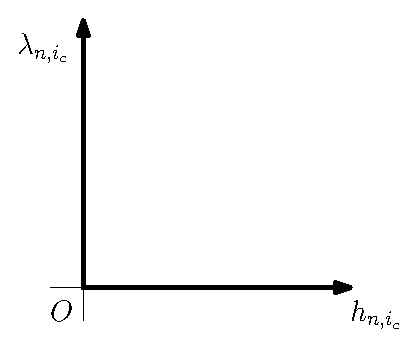
\includegraphics[width=\linewidth]{signorinicontact.eps}
\caption{}\label{fig:signorinicontact}
\end{subfigure}
\qquad
%\begin{subfigure}{0.3\textwidth}
%\centering
%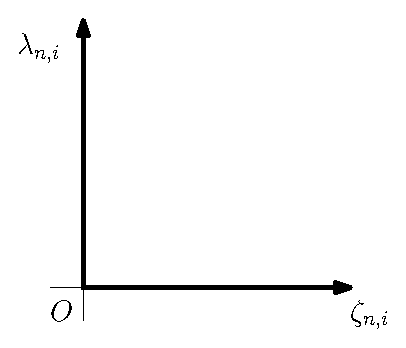
\includegraphics[width=\linewidth]{signoriniforce.eps}
%\caption{Signorini's force law.}\label{fig:signoriniforce}
%\end{subfigure}
%\quad
\begin{subfigure}{0.3\textwidth}
\centering
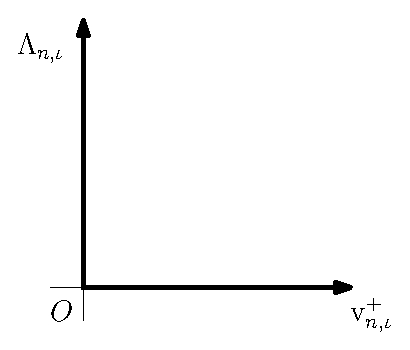
\includegraphics[width=\linewidth]{newtonimpact.eps}
\caption{}\label{fig:newtonimpact}
\end{subfigure}
\caption{In \textnormal{(a)} Signorini's contact law and in \textnormal{(b)} Newton's impact law without restitution.}
\end{figure}
Newton's impact law relates the normal velocities at the contact points after impact to the normal velocities just before the impact using a so-called coefficient of restitution $e$. Mathematically, Newton's impact law can be expressed as
\begin{align}
\vrm^+_{n,\iota} = -e_{n,\iota}\vrm^-_{n,\iota},\text{ when }\hrm_{n,\iota}=0,\ \dot{\hrm}_{n,\iota}<0,
\end{align}
\nomenclature[Ren]{$e_{n,\iota}$}{The normal restitution coefficient of contact point $\iota$}%
\nomenclature[Ret]{$e_{t,\iota}$}{The tangential restitution coefficient of contact point $\iota$}%
where $\vrm^-_{n,\iota}$ and $\vrm^+_{n,\iota}$ are the ante- and post-impact relative normal velocities, respectively, associated with contact point $\iota$. In this work, the coefficient of restitution $e_{n,\iota}$ is assumed to be $0$ for all $\iota$, corresponding to a completely inelastic impact. For closed contacts, an impact law can be defined that relates the impulsive contact force $\Lambda_{n,\iota}$ to the post-impact normal velocity $\vrm_{n,\iota}$. Considering multi-contact systems, two situations can occur when a contact is closed:
\begin{enumerate}
\item $\Lambda_{n,\iota} > 0\ \wedge\ \vrm^+_{n,\iota} = 0$ ($\iota$ participating in impact)
\item $\Lambda_{n,\iota} = 0\ \wedge\ \vrm^+_{n,\iota} \geq 0$ ($\iota$ not participating in impact)
\end{enumerate}
The situations described above are illustrated in Figure~\ref{fig:newtonimpact}, where again the orthogonality can be observed. The behavior can be summarized in the complementarity condition
\begin{align}
0\leq \vrm^+_{n,\iota}\ \bot\ \Lambda_{n,\iota} \geq 0,\quad  \qquad \forall \iota\in\Ic_{\text{cl}},\label{eq:newton}
\end{align}
with $\Ic_{\text{cl}}$ the set of closed contacts. The complementarity condition \eqref{eq:newton} is called Newton's impact law. Note that the impact law is defined on velocity level, whereas the contact law is defined on position level.

\subsection{Coulomb's friction law}\label{sec:2fric}
Coulomb's friction law is often used to model dry friction in mechanical systems. When considering isotropic friction in 3-dimensional environments, Coulomb's friction law states that the tangential reaction force vector at contact point $\iota$ satisfies the inclusion
\begin{align}
-\lambdab_{t,\iota}\ \in\ \left\{ \begin{array}{lll}
||\vbf_{t,\iota}||=0 & \Rightarrow & ||\lambdab_{t,\iota}||\leq\mu_{\iota}\lambda_{n,\iota}\\
||\vbf_{t,\iota}||>0 & \Rightarrow & \lambdab_{t,\iota} = \mu_{\iota}\lambda_{n,\iota}\frac{\vbf_{t,\iota}}{||\vbf_{t,\iota}||}
\end{array}\right.,\label{eq:frictionlen}
\end{align}
\nomenclature[G12]{$\mu_{\iota}$}{The friction coefficient of contact point $\iota$}%
with $\mu_{\iota}$ the friction coefficient at contact point $\iota$. The behavior described in \eqref{eq:frictionlen} can conveniently be described using the normal cone formulation \cite[Section 5.3.2]{Leine2008}. The set of admissible friction forces $C_{t,\iota}\subset\Rbb^2$, which for isotropic friction is a disk given by
\begin{align}
C_{t,\iota} = \left\{-\lambdab_{t,\iota}\ |\ ||\lambdab_{t,\iota}|| \leq \mu_{\iota}\lambda_{n,\iota}\right\}.
\end{align}
The spatial Coulomb's friction law can then given be formulated as
\begin{align}
\vbf_{t,\iota} &\in \mu\lambda_{n,\iota}N_{C_{t,\iota}}(-\lambdab_{t,\iota}),\label{eq:2vNC}
\end{align}
where $N_{C_{t,\iota}}$ is the normal cone set of $C_{t,\iota}$. The normal cone set $N_{C}$ of a convex set $C$ is given by
\begin{align}
N_{C}(\xb) := \left\{\yb\ |\ \yb^T(\xb^\ast-\xb)\leq 0,\quad \xb\in C,\ \forall\xb^\ast\in C \right\}.
\end{align}

\begin{figure}[bt!]
\centering
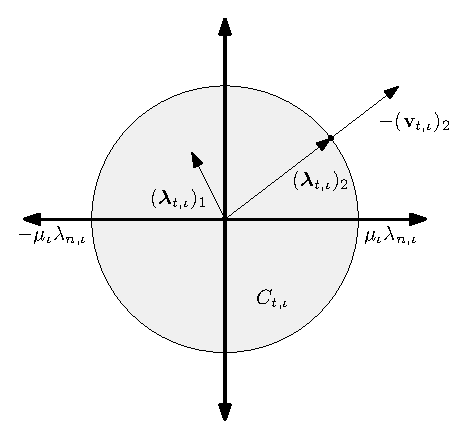
\includegraphics[width=.4\textwidth]{2frictiondisk.eps}\caption{The friction disk with two seperate friction forces $\lambdab_{t,1}$ and $\lambdab_{t,2}$. $\lambdab_{t,1} = \mu\lambda_{n,1}$, resulting in a tangential velocity $\zetab_{t,i}>0$. $\lambdab_{t,2}<\mu\lambda_{n,2}$, leading to a tangential velocity $\zetab_{t,i}=0$.}\label{fig:2frictiondisk}
\end{figure}

The normal cone set $N_{C}(\xb) = 0,\ \forall\xb\in C\setminus \partial C$, where $\partial C$ denotes the boundary of $C$. $N_{C}(\xb) \neq 0,\ \forall\xb\in \partial C$. For all $\xb$ on the boundary of $C$, $N_{C}(\xb)$ consists of the normal cone to the boundary of $C$ on the point $\xb$. The normal cone set can be explained more intuitively using Figure~\ref{fig:2frictiondisk}. We consider two situations: situation one, where $||(\lambdab_{t,\iota})_1|| < \mu_{\iota}\lambda_{n,\iota}$, and situation two, where $||(\lambdab_{t,\iota})_2|| = \mu_{\iota}\lambda_{n,\iota}$. In situation one, $(\lambdab_{t,\iota})_1 \in C_{t,\iota}\setminus \partial C_{t,\iota}$, meaning that $(\vbf_{t,\iota})_1 = 0$ according to \eqref{eq:2vNC}. In situation two, $(\lambdab_{t,\iota})_2 \in \partial C_{t,\iota}$, meaning that $(\vbf_{t,\iota})_2$ is somewhere in the normal cone of $\partial C_{t,\iota}$ at $-\lambdab_{t,\iota}$. When the boundary of $\partial C_{t,\iota}$ is smooth at $-\lambdab_{t,\iota}$, the normal cone $N_{C_{t,\iota}}(-\lambdab_{t,\iota})$ is actually a ray. While the normal cone $N_C$ is also defined for nonsmooth boundaries of $C$, this situation is not considered as the boundary of the set of admissible friction forces $\partial C_{t,\iota}$ is smooth everywhere. The relative tangential velocity $\vbf_{t,\iota}$ is therefore somewhere in the direction of $-\lambdab_{t,\iota}$, which is equivalent to the desired behavior described in \eqref{eq:frictionlen}, i.e.,
\begin{align}
\vbf_{t,\iota} &\in \mu\lambda_{n,\iota}N_{C_{t,\iota}}(-\lambdab_{t,\iota}) \Leftrightarrow -\lambdab_{t,\iota} \in \left\{ \begin{array}{lll}
||\vbf_{t,\iota}||=0 & \Rightarrow & ||\lambdab_{t,\iota}||\leq\mu_{\iota}\lambda_{n,\iota}\\
||\vbf_{t,\iota}||>0 & \Rightarrow & \lambdab_{t,\iota} = \mu_{\iota}\lambda_{n,\iota}\frac{\vbf_{t,\iota}}{||\vbf_{t,\iota}||}
\end{array}\right. .\label{eq:frictiondir}
\end{align}
\nomenclature[G10]{$\kappa_{\iota}$}{Magnitude of the tangential velocity of contact point $\iota$}%
The work in \cite{Anitescu2006} shows a complementarity formulation that is algebraically equivalent to \eqref{eq:2vNC}. This formulation is given by
\begin{align}
&\vbf_{t,\iota}||\lambdab_{t,\iota}|| = -\kappa_{\iota}\lambdab_{t,\iota},\label{eq:coulomb1}\\
&0\leq \mu_{\iota}\lambda_{n,\iota} - ||\lambdab_{t,\iota}||\ \bot\ \kappa_{\iota} \geq 0,\label{eq:coulomb2}
\end{align}
where $\kappa_{\iota}$ is a variable that determines the length of the velocity vector $\vbf_{t,\iota}$. Equations \eqref{eq:coulomb1}-\eqref{eq:coulomb2} will be used in this work to model spatial coulomb friction. We employ again Newton's impact law for modeling the impact behavior where now the tangential contact velocities before and after impact are related to each other using
\begin{align}
\vbf^+_{t,\iota} = -e_{t,\iota}\vbf^-_{t,\iota},
\end{align}
where $e_{t,\iota}$ is the tangential coefficient of restitution that we consider to be zero in this work. Then, similarly to the non-impulsive case, the impulsive Coulomb's friction law can be expressed as
\begin{align}
&\vbf_{t,\iota}^+||\Lambdab_{t,\iota}|| = \kappa_{\iota}\Lambdab_{t,\iota},  &\forall \iota\in\Ic_{\text{cl}},\label{eq:coulombimp1}\\
&0 \leq \mu\Lambda_{n,\iota} - ||\Lambdab_{t,\iota}||\ \bot\ \kappa_{\iota} \geq 0. &\forall \iota\in\Ic_{\text{cl}}.\label{eq:coulombimp2}
\end{align}
Note that, just as the impulsive dynamics in the normal direction, the impulsive friction law only applies to closed contacts.

\subsection{System dynamics with contact and friction law}\label{sec:2contfric}
When the contact and friction laws \eqref{eq:signorini}, \eqref{eq:coulomb1} and \eqref{eq:coulomb2} introduced in Sections~\ref{sec:2cont} and \ref{sec:2fric} are incorporated in the flow dynamics \eqref{eq:appcont1} of the system, a complete model for the continuous dynamics is found, i.e.,
\begin{align}
&\Mb(\qb)\dot{\nub} + \Cb(\qb,\nub) = \Sb(\qb)\ub + \sum_{\iota\in\Ic_{\text{cl}}}\wb_{n,\iota}(\qb)\lambda_{n,\iota} + \Wb_{t,\iota}(\qb)\lambdab_{t,\iota}, \label{eq:ncpcontact1}\\
&0\leq \hrm_{n,\iota}\ \bot\ \lambda_{n,\iota} \geq 0,\label{eq:ncpcontact2}\\
&\vbf_{t,\iota}||\lambdab_{t,\iota}|| = -\kappa_{\iota}\lambdab_{t,\iota},\label{eq:ncpcontact3}\\
&0\leq \mu\lambda_{n,\iota} - ||\lambdab_{t,\iota}||\ \bot\ \kappa_{\iota} \geq 0,\label{eq:ncpcontact4}
\end{align}
with 
\begin{align}
&\hrm_{n,\iota} := \hrm_{n,\iota}(\qb),\label{eq:h}\\
&\vrm_{n,\iota} := \wb^T_{n,\iota}(\qb) \nub,  \label{eq:zetan}\\
&\vbf_{t,\iota} := \Wb^T_{t,\iota}(\qb) \nub. \label{eq:zetab}
\end{align}
Similarly, incorporating the impulsive contact and friction laws \eqref{eq:newton}, \eqref{eq:coulombimp1}, and \eqref{eq:coulombimp1} in the impact/discrete dynamics \eqref{eq:appimp1} gives a complete model for the impact behavior of the system. It follows that the discrete dynamics that are triggered by the occurrence of an impact event are given by
\begin{align}
&\Mb(\qb)(\nub^+ - \nub^-) = \sum_{\iota\in\Ic_{\text{cl}}} \wb_{n,\iota}(\qb)\Lambda_{n,\iota} + \Wb_{t,\iota}(\qb)\Lambdab_{t,\iota}, \label{eq:ncpimpact1}\\
&0\leq \vrm_{n,\iota}^+\ \bot\ \Lambda_{n,\iota} \geq 0, &\forall \iota\in\Ic_{\text{cl}},\label{eq:ncpimpact2}\\
&\vbf_{t,\iota}^+||\Lambdab_{t,\iota}|| = \kappa_{\iota}\Lambdab_{t,\iota},  &\forall \iota\in\Ic_{\text{cl}},\label{eq:ncpimpact3}\\
&0 \leq \mu\Lambda_{n,\iota} - ||\Lambdab_{t,\iota}||\ \bot\ \kappa_{\iota} \geq 0. &\forall \iota\in\Ic_{\text{cl}},\label{eq:ncpimpact4}
\end{align}
with 
\begin{align}
\vrm^+_{n,\iota} &:= \wb^T_{n,\iota}(\qb) \nub^+,\\
\vbf^+_{t,\iota} &:= \Wb^T_{t,\iota}(\qb) \nub^+.\label{eq:ncpimpactend}
\end{align}

\section{Hybrid system formulation}
In this section, the dynamics of the complementarity system defined in Section~\ref{sec:comp} is written to a hybrid formulation, resulting in a hybrid framework for mechanical systems with unilateral constraints and spatial friction. In \cite[p. 222]{Acary2008}, event driven numerical methods are presented for mechanical systems with spatial friction. The model presented in this section is suitable for the simulation methods presented in \cite{Acary2008}.

\nomenclature[G18]{$\sigma_j$}{The system-mode descriptor of event $j$}%
\subsection{Hybrid systems with impulsive effects}\label{sec:2hyb}
According to \cite{Haddad2006}, an impulsive dynamical system can be described by a hybrid system with impulsive effects. This makes it a valid framework for mechanical systems with unilateral constraints and spatial friction. A hybrid system with impulsive effects consists of three elements:
\begin{enumerate}
\item Continuous dynamics, a continuous-time differential equation which defines the behavior of the system in between events
\item Discrete dynamics, a discrete map which defines the way the state of the system is reset during events
\item A criterion to decide when the state of the system is to be reset
\end{enumerate}

The continuous dynamics of the hybrid system with impulsive effects are given by
\begin{align}
\dot{\xb}_j =\fb_j(\xb_j,\ub_j,t), \qquad\xb_j,\ub_j\in \mathcal{C}_j,\label{eq:hybimp1}
\end{align}
with the state $\xb_j = \xb(t,j)\in\Rbb^{n(j)}$ and the input $\ub_j = \ub(t,j)\in\Rbb^{m(j)}$. The nonlinear function $\fb_j:\Rbb^{n(j)}\ \times\ \Rbb^{m(j)}\ \times\ \Rbb\rightarrow \Rbb^{n(j)}$ is a vector field which describes the flow of segment $j$. Here $j\in\{0,1,\dots,N\}$ is a counter that defines the flow set $\mathcal{C}_j$ in which the system resides, where $N$ is the number of segments in a trajectory. When $j$ is increased, and another flow set is entered, the vector field that defines the behavior of the system can change. We refer to $(t,j)$ as the \textit{hybrid time}. Note that the state dimension $n(j)$ and the input dimension $m(j)$ can vary in different segments $j$.

The discrete dynamics of the hybrid system with impulsive effects are given by
\begin{align}
\xb_{j+1} = \gb_j(\xb_j,\ub_j,t), \qquad\xb_j,\ub_j\in \mathcal{D}_{j+1}\label{eq:hybimp2}
\end{align}
The discrete dynamics $\gb_j:\Rbb^{n(j-1)}\ \times\ \Rbb^{m(j-1)}\ \times\ \Rbb\rightarrow \Rbb^{n(j)}$ is a mapping function, which maps the ante-event state to the post-event state. This map is evaluated when the system enters the set $\mathcal{D}_{j+1}(t) \subseteq \partial \mathcal{C}_j := \{\xb(t,j)\in\Rbb^{n(j)},\ \ub(t,j)\in\Rbb^{m(i)}\ |\ \gamma_{j+1}(\xb^{\wedge},\ub^{\wedge},t) = 0\}$, indicating that an event should occur. The set $\mathcal{D}_{j+1}$ is defined using some virtual state and input $\xb^{\wedge}$, $\ub^{\wedge}$ that are not necessarily physically realistic, and a \textit{guard function} $\gamma_{j+1}$. A guard function is a state-and-input dependent differentiable function with the properties
\begin{align}
&\gamma_{j+1}(\xb,\ub,t) > 0,	&(\xb,\ub,t) &\in \mathcal{C}_j\setminus\partial \mathcal{C}_j,\\
&\gamma_{j+1}(\xb,\ub,t) = 0,	&(\xb,\ub,t) &\in \mathcal{D}_{j+1} = \partial \mathcal{C}_j,\\
&\gamma_{j+1}(\xb,\ub,t) < 0,	&(\xb,\ub,t) &\in (\Rbb^n \times \Rbb^m \times \Rbb)\setminus \mathcal{C}_j,
\end{align}
where $\partial \mathcal{C}_j$ is the boundary of flow set $\mathcal{C}_j$. Using a guard function, $\mathcal{C}_j$ and $\mathcal{D}_{j+1}$ can conveniently be described. This is illustrated in Figure~\ref{fig:2guards}. While the guard function is greater than zero, the continuous dynamics \eqref{eq:hybimp1} should be evaluated, since the system is in the interior of flow set $\mathcal{C}_j$. When the guard function is activated, i.e., $\gamma_{j+1} = 0$, the ante-event state $\xb_j(t_{j+1})$ is mapped to the post-event state $\xb_{j+1}(t_{j+1})$ using the discrete dynamics \eqref{eq:hybimp2}. Here $t_{j+1}$ denotes the time-instant where $\gamma_{j+1}$ is activated. After this event, the system will continue flowing in $\mathcal{C}_{j+1}$ according to the vector field $\fb_{j+1}$.

\begin{figure}[bt!]
\centering
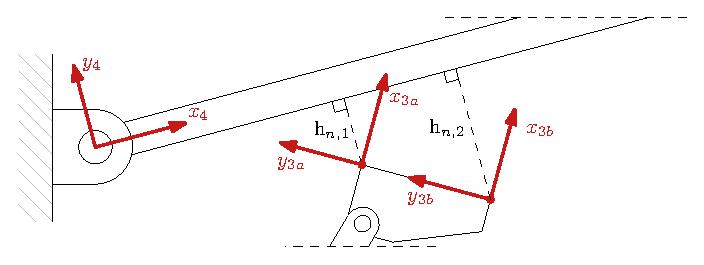
\includegraphics[width=.4\textwidth]{guards.eps}\caption{A guard function defining the flow set $\mathcal{C}_j$ for a 2-dimensional system is illustrated in this figure.} \label{fig:2guards}
\end{figure}

The hybrid dynamics \eqref{eq:hybimp1},\eqref{eq:hybimp2} will form the starting point in formulating the tracking problem for mechanical systems with unilateral constraints and spatial friction. In this, consider a nominal state-and-input trajectory $(\alphab(t,j),\mub(t,j))$ that is a solution to \eqref{eq:hybimp1},\eqref{eq:hybimp2} for initial condition $\alphab(t_0,0) = \alphab_0\in \mathcal{C}_0$ and consists of $N+1$ absolutely continuous segments discriminated by the event counter $j\in\{0,1,\dots,N\}$. The nominal event time of event $j$ is denoted $\tau_j$ and regular time is denoted $t$. An example of a reference trajectory is illustrated in Figure~\ref{fig:2example}.

The figure shows a block that impacts the ground, slides over the ground, and is subsequently lifted from the ground. The block has two contact points on its edges $\iota_1$ and $\iota_2$. The motion starts with both contact points open as can be seen in Figure~\ref{fig:2example1}. The flow is described by $\dot{\alphab}(t,0) = \fb_0(\alphab(t,0),\mub(t,0),t)$ for $t\in[t_0,\tau_1]$. Then, contact is established at contact point $\iota_2$ at the time $\tau_1$, causing a jump in the state and a change in continuous dynamics to the vector field $\fb_1(\alphab(t,1),\mub(t,1),t)$ for $t\in[\tau_1,\tau_2]$. This is illustrated in Figure~\ref{fig:2example2}, where $\iota_2$ is closed and slipping over the contact surface. At the time $\tau_2$, another corner of the rectangle, i.e. contact point $\iota_1$, impacts the ground as well causing another jump and another change in continuous dynamics. The block now has both contact points slipping over the contact surface. After this, both contact points release contact one by one. Since there are no impulsive forces present in this transition, the state does not jump when a contact point releases. However, due to frictional effects, a jump in the time-derivate of the state is possible, which makes these transitions continuous but nonsmooth.

\begin{figure}[bt!]
\centering
\begin{subfigure}[b]{0.17\textwidth}
\centering
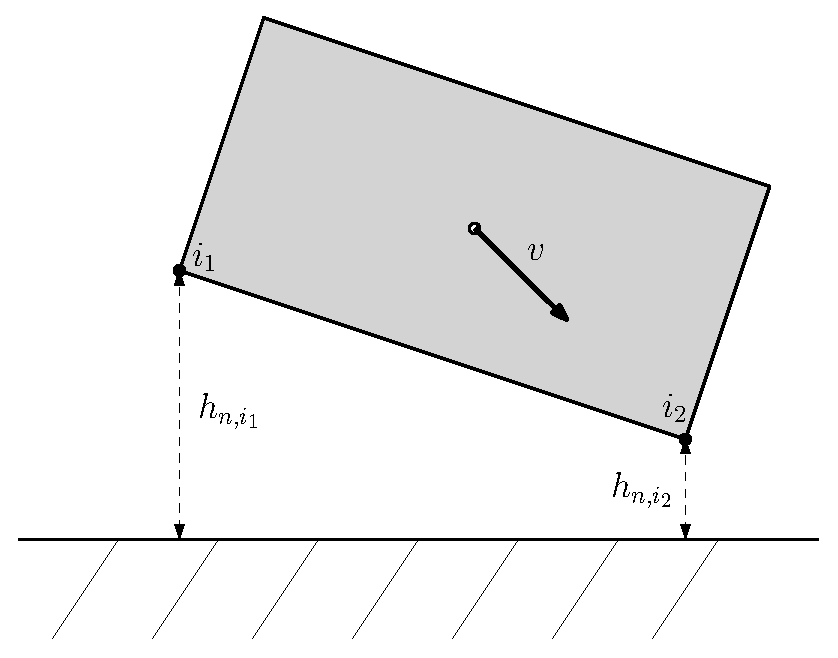
\includegraphics[width=\textwidth]{example1.eps}
\caption{$\begin{array}{l}
\iota_1,\iota_2\in\Ic_{\textnormal{op}}\\ \ls
\end{array}$}
\label{fig:2example1}
\end{subfigure}
\quad
\begin{subfigure}[b]{0.17\textwidth}  
\centering 
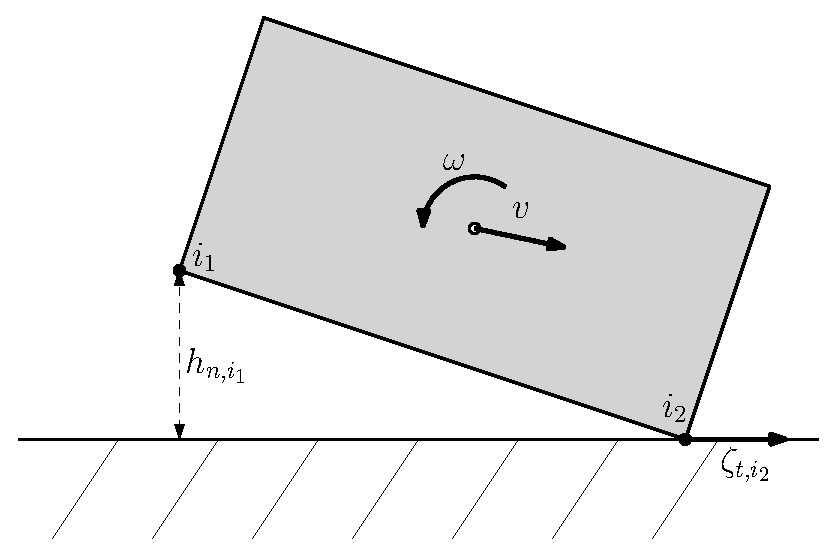
\includegraphics[width=\textwidth]{example2.eps}
\caption{$\begin{array}{l}
\iota_1\in\Ic_{\textnormal{op}}\\\iota_2\in\Ic_{\textnormal{sl}}
\end{array}$}
\label{fig:2example2}
\end{subfigure}
\quad
\begin{subfigure}[b]{0.17\textwidth}   
\centering 
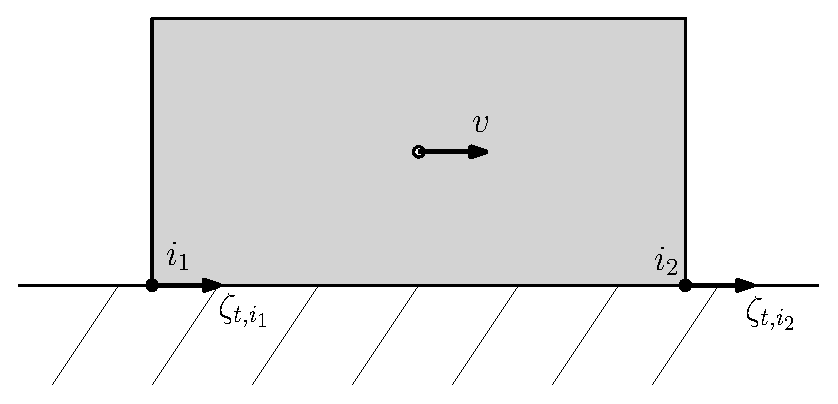
\includegraphics[width=\textwidth]{example3.eps}
\caption{$\begin{array}{l}
\iota_1,\iota_2\in\Ic_{\textnormal{sl}}\\ \ls
\end{array}$}
\label{fig:2example3}
\end{subfigure}
\quad
\begin{subfigure}[b]{0.17\textwidth}  
\centering 
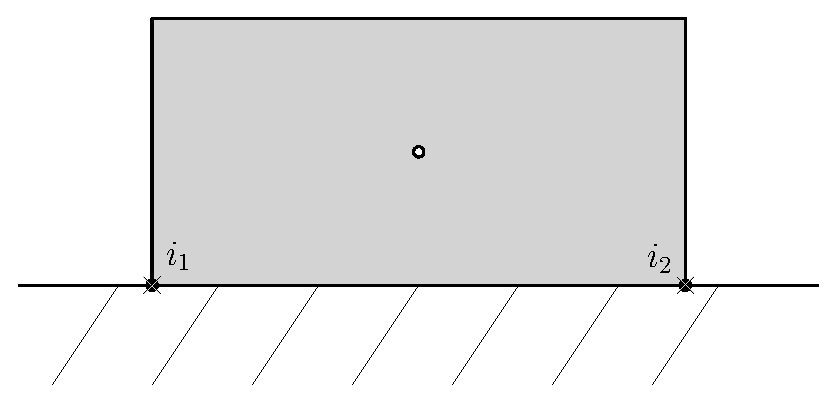
\includegraphics[width=\textwidth]{example4.eps}
\caption{$\begin{array}{l}
\iota_1\in\Ic_{\textnormal{sl}}\\\iota_2\in\Ic_{\textnormal{op}}
\end{array}$}
\label{fig:2example4}
\end{subfigure}
\quad
\begin{subfigure}[b]{0.17\textwidth}   
\centering 
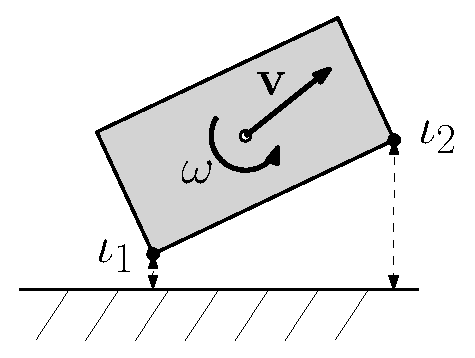
\includegraphics[width=\textwidth]{example5.eps}
\caption{$\begin{array}{l}
\iota_1,\iota_2\in\Ic_{\textnormal{op}}\\ \ls
\end{array}$}
\label{fig:2example5}
\end{subfigure}
\vskip\baselineskip
\begin{subfigure}[b]{\textwidth}   
\centering 
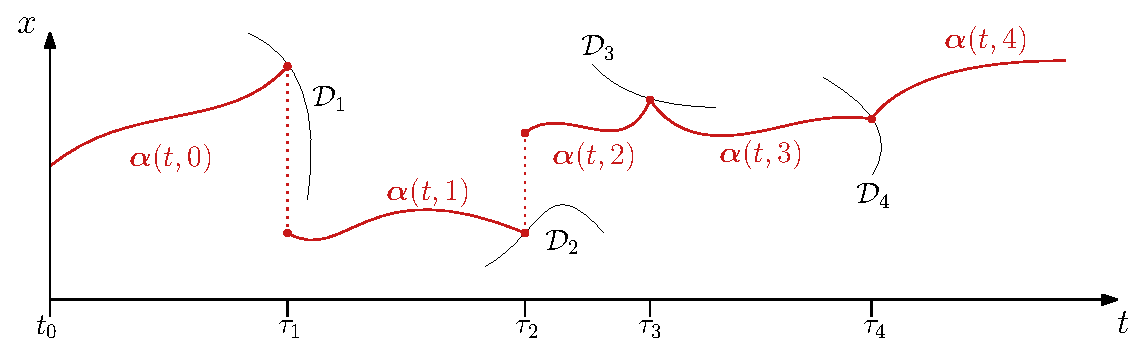
\includegraphics[width=.85\textwidth]{exampletraj1.eps}
\label{fig:2exampletraj}
\end{subfigure}
\caption{An example trajectory, which satisfies the dynamics \eqref{eq:hybimp1}-\eqref{eq:hybimp2}, of a block pushing towards and withdrawing from a surface with velocity $\vbf$. Note that the sets $\mathcal{D}$ besides being dependent on $\xb$, are also dependent on $\ub$. Also, although not depicted in this image, the state space of the system varies with every event.}
\label{fig:2example}
\end{figure}

Next, in Sections~\ref{sec:2event}-\ref{sec:2discdyn}, the complementarity system defined in Section~\ref{sec:comp} will be fitted into the hybrid system \eqref{eq:hybimp1},\eqref{eq:hybimp2}. In Section~\ref{sec:2contdyn}, the continuous dynamics $\fb_j$ will be derived for mechanical systems with unilateral constraints and spatial friction. Then, in Section~\ref{sec:2event} the reset set $\mathcal{D}_j$ will be defined. Finally, in Section~\ref{sec:2discdyn} the discrete dynamics $\gb_j$ will be derived. This will fully define the hybrid system with impulsive effects for mechanical systems with unilateral constraints and spatial friction.

\subsection{Continuous dynamics}\label{sec:2contdyn}
Let us start by considering the state $\xb$ to be composed as
\begin{align}
\xb = \begin{bmatrix}
\qb\\ \dot{\qb}
\end{bmatrix}.
\end{align}
As described in Section~\ref{sec:comp}, for mechanical systems a set of contact points $\mathcal{I} = \{\iota_1,\iota_2,\dots,\iota_c\}$ is defined, with $c$ is the number of considered contact points. A set $\Ic_{\text{cl}}$ is defined as the set of closed contact points, such that a contact $\iota\in\Ic_{\text{cl}}$ has closed a unilateral constraint. The set of contact points in open contact is defined as $\Ic_{\text{op}} := \{\iota\ |\ \iota\notin\Ic_{\text{cl}}\}$. The set $\Ic_{\text{cl}}$ is divided in the subsets $\Ic_{\text{sl}}$ and $\Ic_{\text{st}}$, where $\Ic_{\text{sl}}$ is the set of closed contact points in slip and $\Ic_{\text{st}}$ the set of closed contact points in stick. The division implies that $\Ic_{\text{cl}} =\Ic_{\text{sl}}\cup\Ic_{\text{st}}$ and that $\Ic_{\text{sl}}\cap\Ic_{\text{st}}=\emptyset$. 

The equations of motion, given in \eqref{eq:appcont1}, can be rewritten to
\begin{align}
\dot{\nub} = \Mb^{-1}(\qb)\left[ \Sb(\qb)\ub - \Cb(\qb,\nub) + \Wb_{n}(\qb)\lambdab_{n} + \Wb_{t}(\qb)\lambdab_{t}\right],\label{eq:qddot}
\end{align}
with
\begin{align*}
\Wb_n &= \begin{bmatrix}
\wb_{n,i_1},\wb_{n,i_2},\dots,\wb_{n,\iota}
\end{bmatrix}\in\Rbb^{n\times c},\\
\Wb_t &= \begin{bmatrix}
\Wb_{t,i_1},\Wb_{t,i_2},\dots,\Wb_{t,\iota} 
\end{bmatrix}\in\Rbb^{n\times 2c},\\
\lambdab_n &= \begin{bmatrix}
\lambda_{n,\iota_1};\lambda_{n,\iota_2};...;\lambda_{n,\iota_c} 
\end{bmatrix}\in\Rbb^{c},\\
\lambdab_t &= \begin{bmatrix}
\lambdab_{t,\iota_1};\lambdab_{t,\iota_2};...;\lambdab_{t,\iota_c} 
\end{bmatrix}\in\Rbb^{2c}.
\end{align*}
Note that since $\fb_j$ is only defined on $\xb(t,j),\ub(t,j)\notin \mathcal{D}_{j+1}$, it is not necessary to use $\nub$ to define the equations of motion as done in \eqref{eq:appcont1}. It follows that $\fb_j$ can be written as
\begin{align}
\dot{\xb}_j(t) =\begin{bmatrix}
\dot{\qb}\\ \Mb^{-1}(\qb)\left[ \Sb(\qb)\ub - \Cb(\qb,\dot{\qb}) + \Wb_{n}(\qb)\lambdab_{n} + \Wb_{t}(\qb)\lambdab_{t}\right]
\end{bmatrix}.\label{eq:fcont}
\end{align}
The closed contact points in $\Ic_{\text{cl}}$ experience reaction forces $\lambda_{n,\iota}$ and $\lambdab_{t,\iota}$, as can be seen in \eqref{eq:qddot}. Therefore, for all closed contact points $\iota\in\Ic_{\text{cl}}$, constraints are included which restrict these reaction forces. These constraints are given by
\begin{align}
\wb^T_{n,\iota}(\qb)\ddot{\qb} + \dot{\wb}^T_{n,\iota}(\qb)\dot{\qb} &= 0, &\forall \iota\in\Ic_{\text{cl}},\label{eq:fcontconst1}\\
\lambdab_{t,\iota}||\Wb_{t,\iota}^T\dot{\qb}|| + \mu_{\iota}\lambda_{n,\iota}\Wb_{t,\iota}^T\dot{\qb} &= 0, &\forall \iota\in\Ic_{\text{sl}},\label{eq:fcontconst2}\\
\Wb^T_{t,\iota}(\qb)\ddot{\qb} + \dot{\Wb}^T_{t,\iota}(\qb)\dot{\qb} &= 0, &\forall \iota\in\Ic_{\text{st}},\label{eq:fcontconst3}
\end{align}
where again $\Ic_{\text{sl}}$ and $\Ic_{\text{st}}$ are the sets of closed contacts in slip and closed contacts in stick, respectively. With \eqref{eq:fcont} and \eqref{eq:fcontconst1}-\eqref{eq:fcontconst3}, the continuous dynamics of the hybrid system are correctly defined.

\textbf{System mode descriptor}\\
A system will have different flow dynamics as the system mode changes, as can be seen in \eqref{eq:fcontconst1}-\eqref{eq:fcontconst3}. Also the jump sets $\mathcal{D}_j$ change with the mode, as will be shown in Section~\ref{sec:2event}. Therefore it is necessary to keep track of the mode the system is in. The system mode descriptor $\sigma_j$ is introduced to conveniently describe the current system mode. Each contact point can either be in open-contact, closed-contact slip or closed-contact stick. The system mode descriptor is therefore defined as the ordered set
\begin{align}
\sigma = (\sigma_1,\sigma_2,\dots,\sigma_\iota),
\end{align}
where $\sigma_\iota$ is the mode of contact point $\iota$. $\sigma_\iota$ can either have the value `op' for a contact point in open-contact, `sl' for a contact point in closed-contact slip, or `st' for a contact point in closed-contact stick. For example, the system mode descriptor of the mode in Figure~\ref{fig:2example2} is $\sigma = (\text{op},\text{sl})$.

\subsection{Discrete event sets}\label{sec:2event}
When the system state enters an event set $\mathcal{D}$, an event will take place. The current mode for the different contact points is in that case altered and a corresponding state reset is applied. In this section the sets $\mathcal{D}$ are defined for each mode of a contact point. The derivation of the discrete event sets can be found in Appendix~\ref{app:hybriddisc}. The discrete event sets are defined using guard functions as presented in Section~\ref{sec:2hyb}. Furthermore, in this section the superscript $(\cdot)^{\sigma_\iota^-\rightarrow\sigma_\iota^+}$ is introduced to indicate that the guard function $\gamma^{\sigma_\iota^-\rightarrow\sigma_\iota^+}$, or event set $\mathcal{D}^{\sigma_\iota^-\rightarrow\sigma_\iota^+}$ is related to the transition from ante-event mode $\sigma_\iota^-$ to post-event mode $\sigma_\iota^+$.

\textbf{Discrete events sets in open contact}\\
For all contact points $\iota\in\Ic_{\text{op}}$, the discrete event sets are defined as
\begin{align}
\mathcal{D}^{\text{op}\rightarrow\text{cl}}_{\iota} &= \{ \xb\ |\ \gamma^{\text{op}\rightarrow\text{cl}}_{\iota} = 0 \},\label{eq:2Dopcl}
\end{align}
\nomenclature[RD]{$\mathcal{D}_j$}{The discrete event set of event $j$}%
with
\begin{align}
\gamma^{\text{op}\rightarrow\text{cl}}_{\iota} &= \hrm_{n,\iota}(\qb).
\end{align}


\textbf{Discrete events sets in closed contact slip}\\
For all contact points $\iota\in\Ic_{\text{sl}}$, the discrete event sets are defined as
\begin{align}
\mathcal{D}^{\text{sl}\rightarrow\text{st}}_{\iota} &= \{ \qb\ |\ \gamma^{\text{sl}\rightarrow\text{st}}_{\iota} = 0\},\label{eq:2Dslst}\\
\mathcal{D}^{\text{cl}\rightarrow\text{op}}_{\iota} &= \{ \qb,\ub\ |\ \gamma^{\text{cl}\rightarrow\text{op}}_{\iota} = 0\},\label{eq:2Dslop}
\end{align}
with 
\begin{align}
\gamma^{\text{sl}\rightarrow\text{st}}_{\iota} &= \sqrt{\vbf_{t,\iota}^T\vbf_{t,\iota}},\\
\gamma^{\text{cl}\rightarrow\text{op}}_{\iota} &= \lambda_{n,\iota}.
\end{align}

\textbf{Discrete events sets in closed contact stick}\\
For all contact points $\iota\in\Ic_{\text{st}}$, the discrete event sets are defined as
\begin{align}
\mathcal{D}^{\text{st}\rightarrow\text{sl}}_{\iota} &= \{ \qb,\ub\ |\ \gamma^{\text{st}\rightarrow\text{sl}}_{\iota} = 0 \},\label{eq:2Dstsl}\\
\mathcal{D}^{\text{cl}\rightarrow\text{op}}_{\iota} &= \{ \qb,\ub\ |\ \gamma^{\text{cl}\rightarrow\text{op}}_{\iota} = 0 \},\label{eq:2Dstop}
\end{align}
with 
\begin{align}
\gamma^{\text{st}\rightarrow\text{sl}}_{\iota} &= \mu^2\lambda_{n,\iota}^2-\lambdab_{t,\iota}\lambdab_{t,\iota}^T,\\
\gamma^{\text{cl}\rightarrow\text{op}}_{\iota} &= \lambda_{n,\iota}.
\end{align}

\subsection{Discrete dynamics}\label{sec:2discdyn}
Whenever the state $\xb$ reaches the discrete event set $\mathcal{D}$, continuous evolution in its current mode is generally not feasible. The system should therefore go through a discrete event, in which the state is reinitialized and the mode is changed. One contact point entering a discrete event set can lead to other contact points experiencing infeasible reaction forces, making it difficult to determine in what mode each contact point should be. The reinitialization of the state and selection of a post-event mode is described by the discrete dynamics in this section. First a \textit{nonlinear complementarity problem} (NCP) is solved to reinitialize the state. The NCP generates a unique feasible solution \cite{Delassus1917}, which for simple systems can be found by iterating over all possible modes until the feasible solution is found. Then, a mode selection algorithm is presented to find a feasible post-event mode, which defines the continuous dynamics to be integrated after the event. 
\nomenclature[A]{NCP}{Nonlinear Complementarity Problem}%

\textbf{State reinitialization}\\
From the impulsive dynamics \eqref{eq:ncpimpact1}-\eqref{eq:ncpimpact4}, the discrete dynamics for an impulsive event which determine the post-event joint velocity $\dot{\qb}^+$ can be derived as
\begin{align}
\dot{\qb}^+ &= \Mb^{-1}\left[\Wb_{n}\Lambdab_{n} + \Wb_{t}\Lambdab_{t}\right] + \dot{\qb}^-, \label{eq:2ncp1}\\
\wb^T_{n,\iota}\dot{\qb}^+ &= 0, &\forall \iota\in\Ic_{\text{cl}},\label{eq:2ncp2}\\
\Lambdab_{t,\iota}||\Wb^T_{t,\iota}\dot{\qb}^+|| + \mu\Lambda_{n,\iota}\Wb^T_{t,\iota}\dot{\qb}^+&= 0, &\forall \iota\in\Ic_{\text{sl}},\label{eq:2ncp3}\\
\Wb^T_{t,\iota}\dot{\qb}^+ &= 0, &\forall \iota\in\Ic_{\text{st}}.\label{eq:2ncp4}
\end{align}
Here the unknown variables are $\dot{\qb}^+\in\Rbb^{n}$, $\Lambdab_{n}\in\Rbb^{c_{\text{cl}}}$ and $\Lambdab_{t}\in\Rbb^{2c_{\text{cl}}}$, which means that there are $n+3c_{\text{cl}}$ unknown variables. From \eqref{eq:2ncp1} we get $n$ equations, from \eqref{eq:2ncp2} we get $c_{\text{cl}}$ equations and since $\Ic_{\text{sl}}\cup\Ic_{\text{st}}=\Ic_{\text{cl}}$, $\Lambdab_{t,\iota}\in\Rbb^2$, and $\dot{\Wb}^T_{t,\iota}\dot{\qb}^+ \in\Rbb^2$ we get $2c_{\text{cl}}$ equations from \eqref{eq:2ncp3}-\eqref{eq:2ncp4}. Since we have $n+3c_{\text{cl}}$ unknown variables and $n+3c_{\text{cl}}$ equations, the system is solvable.

The problem that remains is that it is not straightforward to identify what the correct mode and therewith what the sets $\mathcal{I}_{\textnormal{op}}$, $\mathcal{I}_{\textnormal{sl}}$, and $\mathcal{I}_{\textnormal{st}}$ should be after an event. The set of equations that should be solved is the set of equations that corresponds to the system-mode which generates a feasible post-event state. When a contact point enters a discrete event set, and thus generates an infeasible state, it can be concluded that the system will go through an event because in it's current mode the system is infeasible. However, it is not guaranteed that the contact point which entered the event set will change their mode. Actually any contact point, or even several contact points, can change their mode. Therefore the dynamics should be solved for several modes, until a feasible post-event state is found. A feasible post-event state is a post-event state solved for a certain system-mode $\sigma$, such that the all corresponding guard functions are inactive, i.e., all $\Gamma_{\iota}>0$. As mentioned earlier, there will exist a unique system-mode where the system has a feasible post-impact state. Similar to the non-impulsive guard functions defined in Section~\ref{sec:2event}, the impulsive guard functions are given by
\begin{align}
\Gamma^{\text{cl}\rightarrow\text{op}}_{\iota} &= \Lambda_{n,\iota},\\
\Gamma^{\text{sl}\rightarrow\text{st}}_{\iota} &= (\vbf^+_{t,\iota})^T\vbf^+_{t,\iota},\\
\Gamma^{\text{st}\rightarrow\text{sl}}_{\iota} &= \mu^2\Lambda_{n,\iota}^2 - \Lambdab_{t,\iota}\Lambdab_{t,\iota}^T.
\end{align}
Note that all guard functions are defined at velocity level during the state reinitialization. The NCP \eqref{eq:2ncp1}-\eqref{eq:2ncp4} is defined at velocity level, meaning that only guard functions on velocity level need to be considered. For example, it is impossible for the state reinitialization to generate an infeasible position because the position of the system is not updated during the state reinitialization. When $\Lambda_{n,\iota} = 0$ and $\Lambdab_{t,\iota} = 0$ during an event, one speaks of a non-impulsive event. In this case, the state is not reinitialized during the event. However, the system will enter a different mode. For both impulsive and non-impulsive events, the post-event mode is determined during the mode selection, which is described below.

\textbf{Mode selection}\\
The mode $\sigma$ of a system is determined by the guard functions defined in Section~\ref{sec:2event}. All guard functions $\gamma_\iota$ should be greater than zero for the system to be in a feasible mode. Because some of these guard functions are defined on acceleration level and the post-event acceleration is not constrained by the NCP, we should first find a post-event mode $\sigma^+$ where the accelerations $\ddot{\qb}$ and reaction forces $\lambdab_{n},\lambdab_{t}$ are feasible before we know which vector field is suitable to define the next flow phase. From the continuous dynamics \eqref{eq:ncpcontact1}-\eqref{eq:ncpcontact4}, post-event accelerations and reaction forces can be computed from
\begin{align}
\ddot{\qb}^+ &= \Mb^{-1}\left[\Sb\ub^+ - \Cb + \Wb_{n}\lambdab^+_{n} + \Wb_{t}\lambdab^+_{t}\right], &  \label{eq:2nonimp1}\\
\wb^T_{n,\iota}\ddot{\qb}^+ + \dot{\wb}^T_{n,\iota}\dot{\qb}^+ &= 0, & \forall \iota\in\Ic_{\text{cl}},\label{eq:2nonimp2}\\
\lambdab^+_{t,\iota}||\Wb^T_{t,\iota}\dot{\qb}^+|| + \mu\lambda^+_{n,\iota}\Wb^T_{t,\iota}\dot{\qb}^+ &= 0, & \forall \iota\in\Ic_{\text{sl}},\label{eq:2nonimp3}\\
\Wb^T_{t,\iota}\ddot{\qb}^+ + \dot{\Wb}^T_{t,\iota}\dot{\qb}^+ &= 0, & \forall \iota\in\Ic_{\text{st}},\label{eq:2nonimp4}
\end{align}
where $\Mb$, $\Sb$, $\Cb$, $\wb_{n,\iota}$ and $\Wb_{t,\iota}$ are evaluated at the post-event joint configuration $\qb^+$ and velocity $\dot{\qb}^+$. Because we are interested in whether the accelerations and reaction forces are feasible, the guard functions defined on acceleration level are evaluated. The guard functions that determine the feasibility of a post-event mode are given by
\begin{align}
\gamma^{\text{cl}\rightarrow\text{op}}_{\iota} &= \lambda_{n,\iota}, & \forall \iota\in\Ic_{\text{cl}},\\
\gamma^{\text{st}\rightarrow\text{sl}}_{\iota} &= \mu_{\iota}^2\lambda_{n,\iota}^2 - \lambdab_{t,\iota}\lambdab_{t,\iota}^T, & \forall \iota\in\Ic_{\text{st}},
\end{align}
with $\Ic_{\text{sl}}\cup\Ic_{\text{st}}=\Ic_{\text{cl}}$. Note that the guard functions $\gamma_{\iota}^{\text{op}\rightarrow\text{cl}}$ and $\gamma_{\iota}^{\text{sl}\rightarrow\text{st}}$ are not evaluated. This is unnecessary, because open contact points can only trigger guard functions defined at position level. Since the non-impulsive dynamics only update the acceleration, it is impossible for a contact point in open contact to change mode during an impulsive event. This also holds for the guard function from slip to stick, which is defined on velocity level.

The process of solving a hybrid system with impulsive effects is illustrated in Figure~\ref{fig:2hybridalg}. The system first flows according to a vector field $\fb$. When the event set $\mathcal{D}$ is reached, a jump in the system state $\xb$ is applied. This jump is the result of solving an NCP to find the post-event state $\xb^+$. Finally, the mode selection is performed to find a feasible post-event mode $\sigma^+$ for that post-event state $\xb^+$. The continuous dynamics for the next flow segment is defined by $\sigma^+$ with $\xb^+$ as initial condition.

\begin{figure}[bt!]
\centering
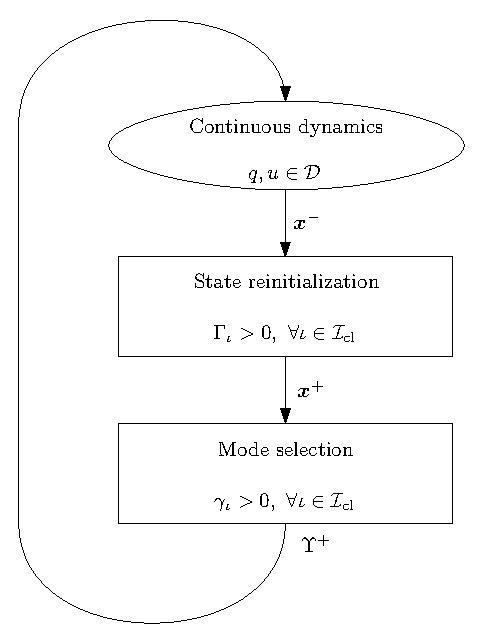
\includegraphics[width=.35\textwidth]{hybridalg.eps}\caption{The algorithm used to solve a hybrid system with impulsive effects depicted in a flowchart.} \label{fig:2hybridalg}
\end{figure}

\section{Summary}
The modeling of mechanical systems with unilateral constraints and spatial friction is presented in this chapter. First, a complementarity problem formulation for such systems is presented using Signorini's contact law, Newton's impact law, and Coulomb's friction law. This system fully defines the dynamics of mechanical systems with unilateral constraints and spatial friction. From the complementarity problem formulation a hybrid system with impulsive effects is derived. This system is constructed with a control point-of-view in mind, and its compatibility with the control strategy that will be presented in the following chapters. The hybrid system is defined in three parts. First the continuous dynamics are presented. Then the discrete event sets are given, which are state-input sets that trigger a discrete event when the state and input enters such a set. Finally, the dynamics of such an event are presented, which consist of a state reinitialization and a mode selection.
\end{document}